\documentclass[border=10pt]{standalone}

\usepackage{tikz}
\usepackage{tikzsymbols}
\usetikzlibrary{calc,patterns,shapes.geometric}

\def\centerarc[#1](#2)(#3:#4:#5){\draw[#1] ($(#2)+({#5*cos(#3)},{#5*sin(#3)})$) arc (#3:#4:#5);}

\begin{document}
	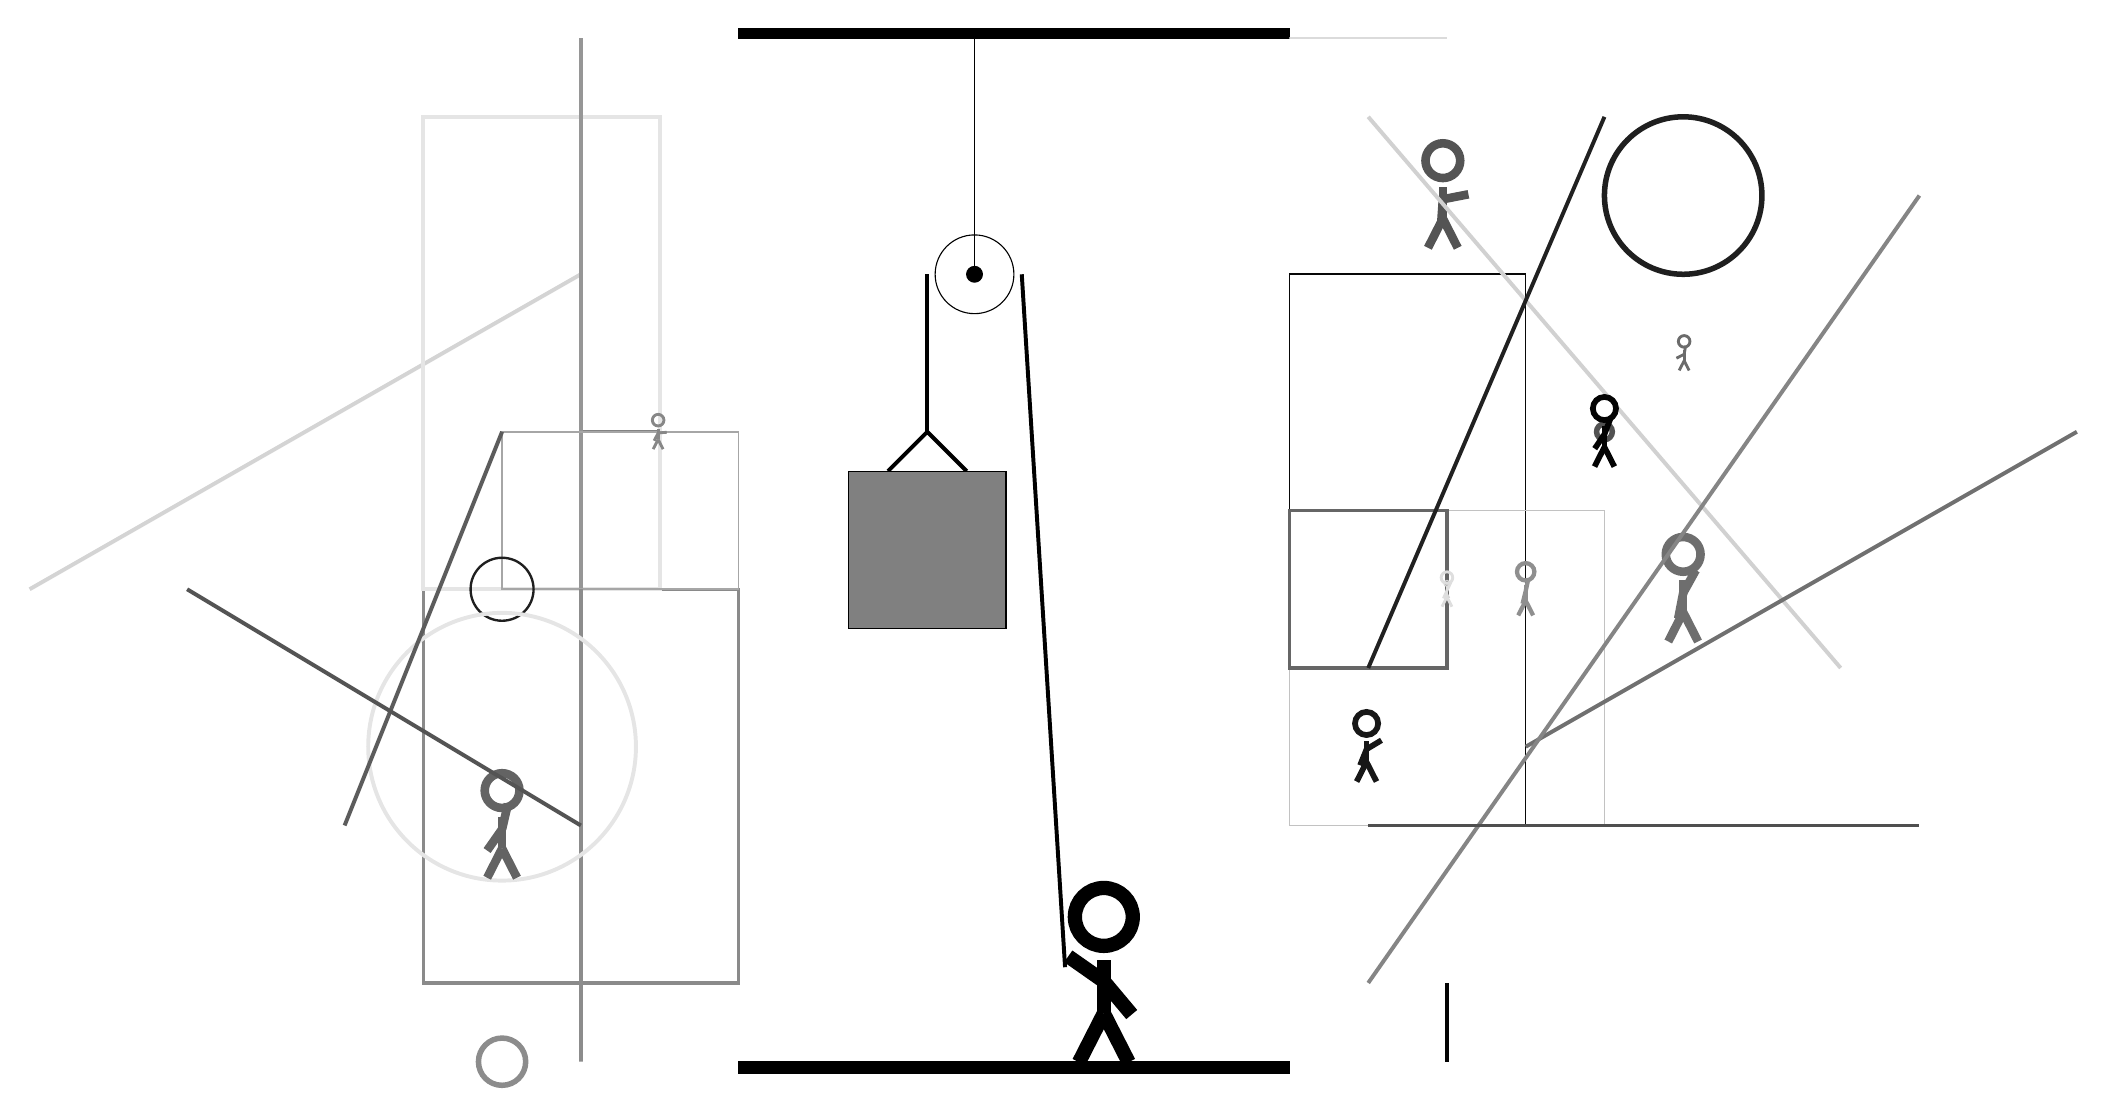
\begin{tikzpicture}
		%%%%% START %%%%%
		
		\draw[fill=black] (-2, 10) rectangle (5, 10.125);
		
		\draw (1, 7) circle (0.5);
		\draw[fill=black] (1, 7) circle (0.1);
		\draw (1, 10) -- (1, 7);
		
		\draw[line width=0.5mm] (-0.1, 4.5) -- (0.4, 5.0) -- (0.9, 4.5);
		\draw[fill=black!50] (-0.6, 4.5) rectangle (1.4, 2.5);
		
		\draw[line width=0.5mm] (0.4, 7) -- (0.4, 5.0);
		\centerarc[line width=0.5mm](1, 7)(0:180:0.6);
		\draw[line width=0.5mm](1.6, 7) -- (2.15, -1.8);
		
		\node at (2.6, -1.9) {\Strichmaxerl[10][-35][-50]};
		
		\draw[line width=0.2mm, color=black!97] (5, 7) rectangle (8, 0);
		
		\draw[line width=0.2mm, color=black!24] (5, 0) rectangle (9, 4);
		\draw [line width=0.7mm, color=black!45](-5, -3) circle (0.3);
		\node[line width=0.2mm, color=black!67] at (7, 8) {\Strichmaxerl[6][86][11]};
		
		\node[line width=0.3mm, color=black!44] at (8, 3) {\Strichmaxerl[3][76][78]};
		
		\draw[line width=0.5mm, color=black!60] (5, 2) rectangle (7, 4);
		\draw[line width=0.5mm, color=black!18](6, 9) -- (12, 2);
		\draw[line width=0.4mm, color=black!46] (-2, -2) rectangle (-6, 3);
		\node[line width=0.6mm, color=black!17] at (7, 3) {\Strichmaxerl[1][77][69]};
		\node[line width=0.2mm, color=black!57] at (10, 3) {\Strichmaxerl[6][79][61]};
		
		\node[line width=0.6mm, color=black!13] at (7, 3) {\Strichmaxerl[2][66][64]};
		
		\draw[line width=0.5mm, color=black!87](9, 9) -- (6, 2);
		\draw[line width=0.5mm, color=black!17](-4, 7) -- (-11, 3);
		
		\draw[line width=0.4mm, color=black!49] (-4, 5) rectangle (-3, 5);
		\draw[line width=0.5mm, color=black!10] (-3, 9) rectangle (-6, 3);
		\draw[line width=0.5mm, color=black!41](-4, 10) -- (-4, 2);
		
		\draw[line width=0.2mm, color=black!35] (-2, 5) rectangle (-5, 3);
		\draw [line width=0.7mm, color=black!68](9, 5) circle (0.1);
		\draw[line width=0.5mm, color=black!56](8, 1) -- (15, 5);
		
		\node[line width=0.2mm, color=black!58] at (10, 6) {\Strichmaxerl[2][27][80]};
		\draw [line width=0.3mm, color=black!88](-5, 3) circle (0.4);
		
		\draw[line width=0.3mm, color=black!14] (7, 10) rectangle (5, 10);
		
		\draw[line width=0.5mm, color=black!48](6, -2) -- (13, 8);
		\node[line width=0.5mm, color=black!99] at (9, 5) {\Strichmaxerl[4][56][69]};
		\draw[line width=0.5mm, color=black!45] (-4, 3) rectangle (-4, -3);
		\node[line width=0.6mm, color=black!47] at (-3, 5) {\Strichmaxerl[2][63][5]};
		\node[line width=0.3mm, color=black!91] at (6, 1) {\Strichmaxerl[4][68][31]};
		\draw[line width=0.5mm, color=black!69](6, 0) -- (13, 0);
		\draw [line width=0.5mm, color=black!10](-5, 1) circle (1.7);
		
		\draw[line width=0.5mm, color=black!99](7, -3) -- (7, -2);
		\draw[line width=0.6mm, color=black!59] (7, 9) rectangle (7, 9);
		\node[line width=0.3mm, color=black!61] at (-5, 0) {\Strichmaxerl[6][55][77]};
		\draw [line width=0.7mm, color=black!88](10, 8) circle (1.0);
		
		\draw[line width=0.5mm, color=black!64](-5, 5) -- (-7, 0);
		\draw[line width=0.5mm, color=black!67](-4, 0) -- (-9, 3);
		
		\draw[fill=black] (-2, -3) rectangle (5, -3.15);
		
		%%%%% END %%%%%
	\end{tikzpicture}
\end{document}